%% LyX 2.0.3 created this file.  For more info, see http://www.lyx.org/.
%% Do not edit unless you really know what you are doing.
\documentclass[english]{article}
\usepackage[T1]{fontenc}
\usepackage{graphicx}
\usepackage{babel}
\usepackage{xunicode}
\begin{document}
I converted the stereographic projection to the HEALPIX map in order
to compare with the original method. The shown results uses a exact
normalization function (sum over the pixels instead of a integral).
The time cost is about 210 secs on my MacBook Pro. While if use a
approximation normalize funtion, the time cost is only 55 secs. The
difference between the result of the new method and original method
is mainly random error. However there is some large difference at
some pixels. I'm still checking what's the problem. Suggestions are
welcome.
\begin{figure}[htbp]
  \centering
  \fbox{
    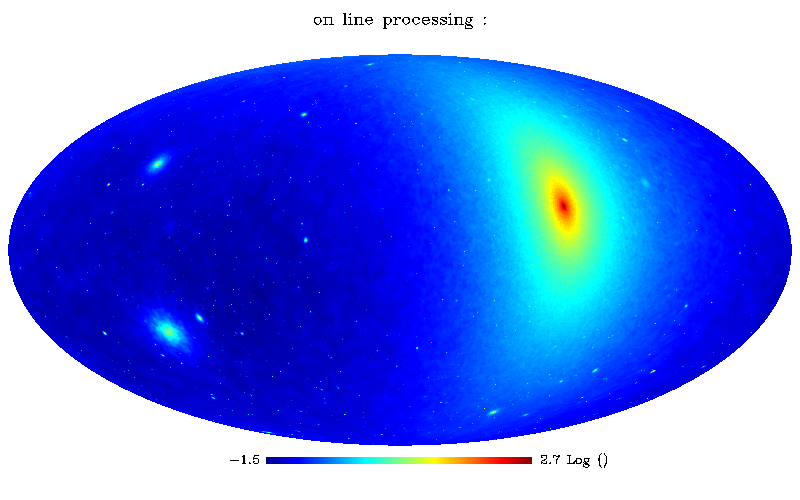
\includegraphics[scale=0.5]{first_run}
  }
  \caption{title}
  \label{labelname}
\end{figure}

\begin{figure}[htbp]
  \centering
  \fbox{
    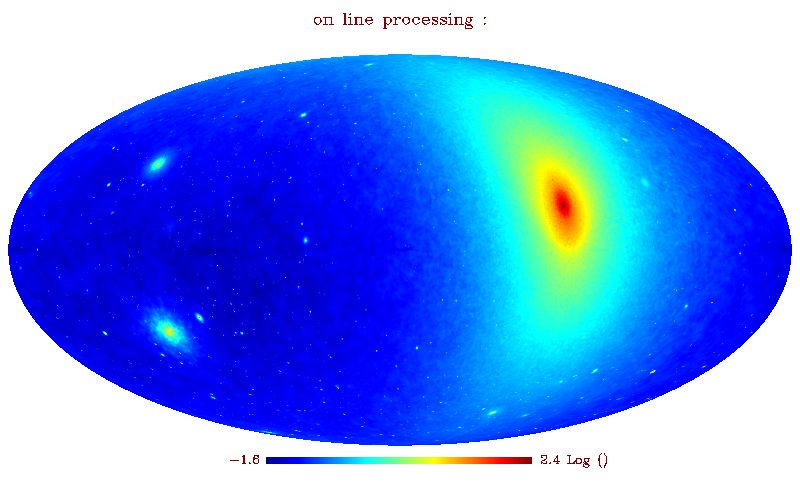
\includegraphics[scale=0.5]{sky}
  }
  \caption{title}
  \label{labelname}
\end{figure}

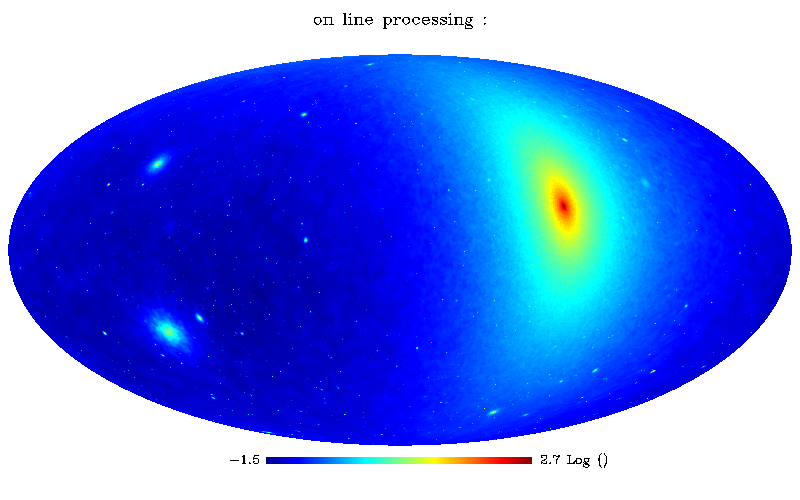
\includegraphics[scale=0.7]{original}

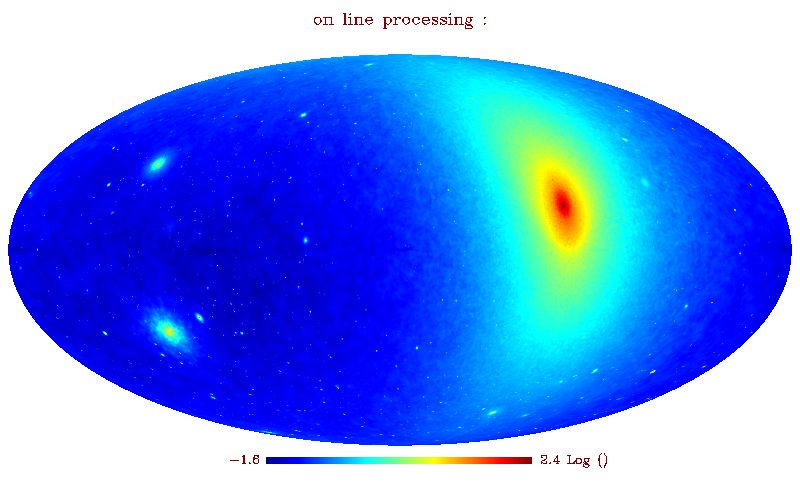
\includegraphics[scale=0.7]{new}

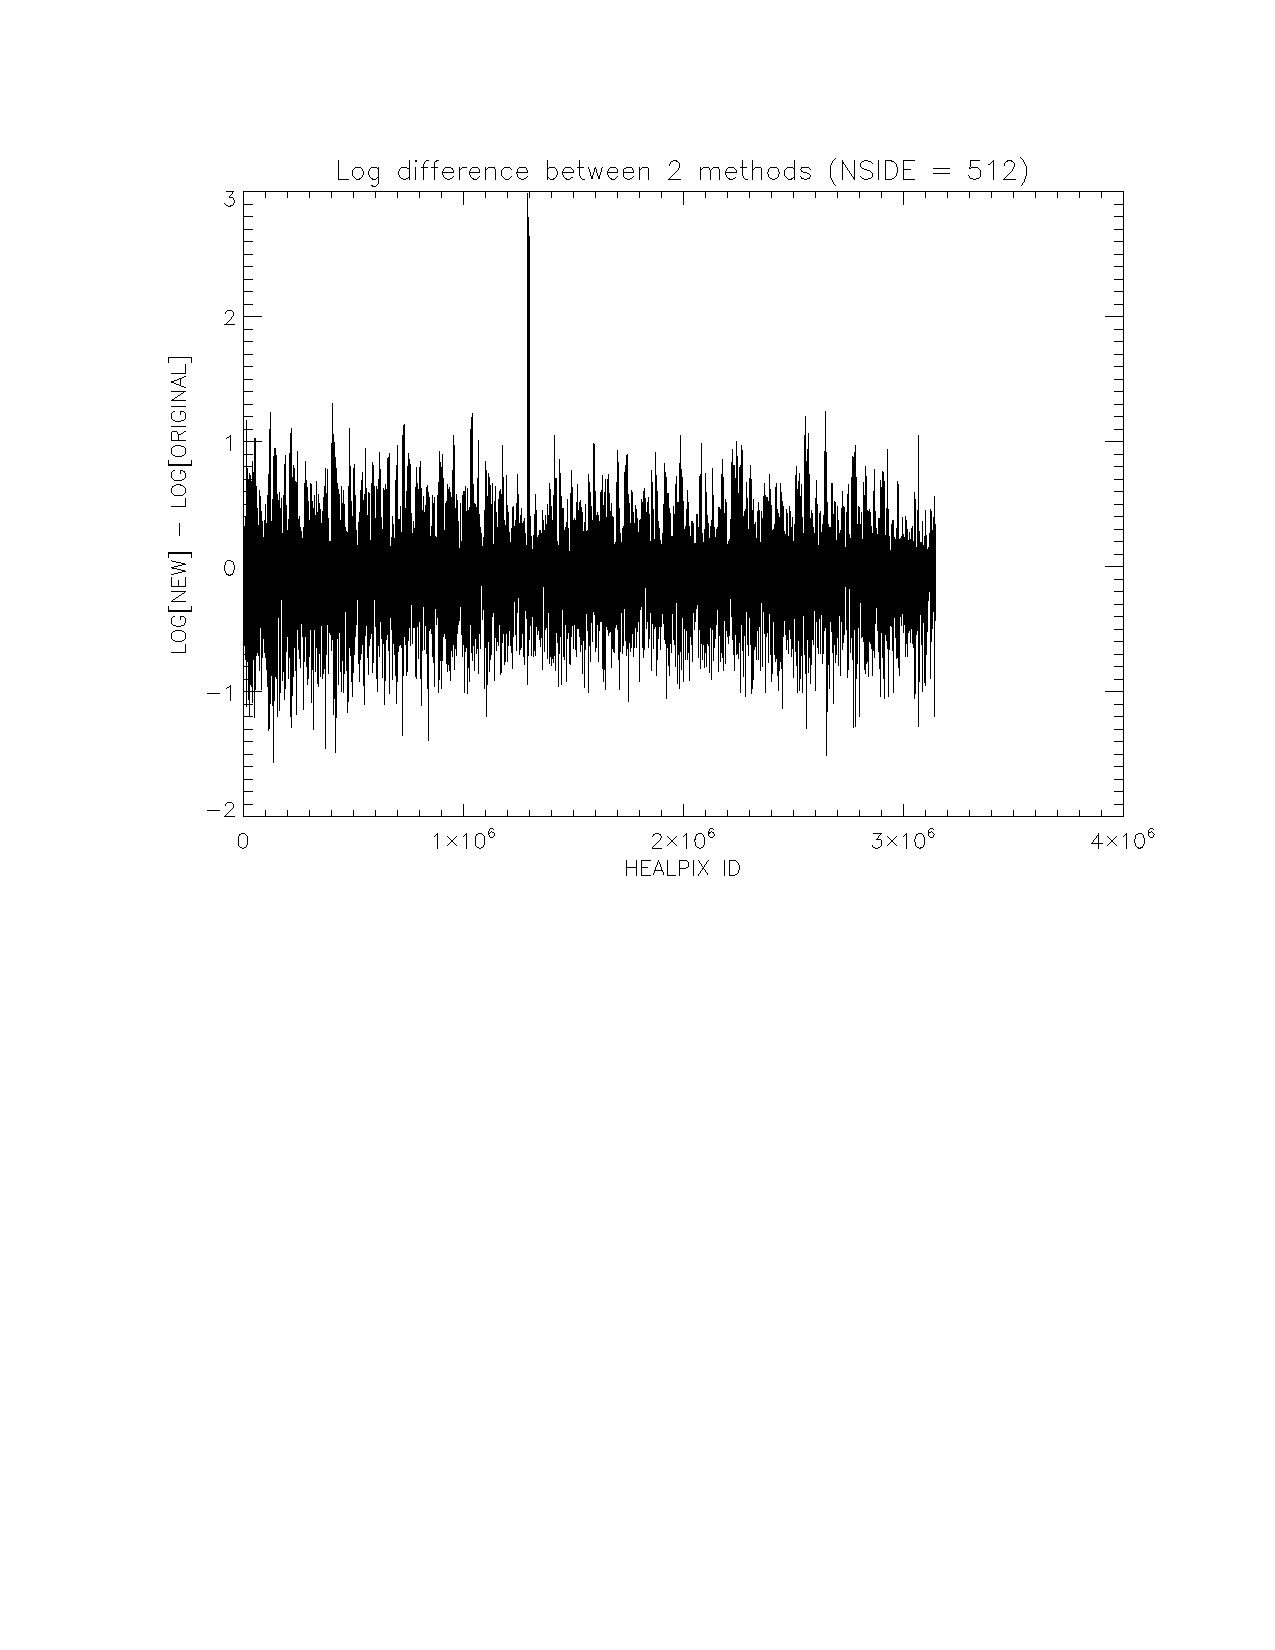
\includegraphics[scale=0.7]{diff.pdf}
\end{document}
